\documentclass[10pt]{book}
\usepackage{cdtBook}
\usepackage{cambios}
\usepackage{usecases}


%\newcommand{\proceso}{Gestión Integral de Residuos Sólidos Urbanos }
\defSistema{SIDAM}

\title{\Sistema \\\LARGE{sistema de rex \\{\bf Prototipo 1}}}
\subtitle{Análisis de Requerimientos}
%\author{}

%\date{martes 11 de mayo de 2010}

%%%%%%%%%%%%%%%%%%%%%%%%%%%%%%%%%%%%%%%%%%%%%%%%%%%%%%%%%%%%%%%%
\begin{document}
\ThisLRCornerWallPaper{0.5}{images/agua.png}
\maketitle\thispagestyle{empty}

\frontmatter
\tableofcontents

\mainmatter


%=========================================================
\chapter{Alcance del prototipo}

	En este capítulo se describe el alcance del prototipo a desarrollar. El alcance del sistema se ha definido como se muestra en la figura~\ref{fig:casosDeUsoCompleto} en donde cada módulo se describe a continuación.



\begin{description}
	\item[Secretaría:] Incluye toda la funcionalidad para que la dirección pueda definir los Programas de la Secretaría y monitorearlos en un nivel muy general. El monitoreo incluye: avances, estado financiero global, semáforos y notas dirigidas a la gerencia. Así como la definición de Temas Transversales y Ejes temáticos.
	\item[Gerencia:] Incluye la funcionalidad para definir, actualizar y monitorear los programas y proyectos contemplados en cada Programa. Así como la definición de fechas y periodos para actualización de información por parte de los coordinadores.
	\item[Coordinación:] Incluye la definición de acciones, indicadores tanto físicos como financieros y metas para los proyectos asignados. Así como el reporte de avances de los proyectos y el registro de estudios derivados del proyecto.
	\item[Mensajes y Notificaciones:] Permite la comunicación en el sistema de los usuarios de una manera jerárquica por medio de mensajes simples.
	\item[Consulta Ciudadana:] Incluye el acceso a la información de los proyectos y los estudios realizados por parte del público en general.
	\item[Administración:] Administración de cuentas de usuarios y mantenimiento a los catálogos del sistema.
\end{description}

\section{Actores}

El sistema será usado por los usuarios cuyos perfiles se describen en la figura~\ref{fig:actores}.

\begin{figure}[htbp!]
	\begin{center}
		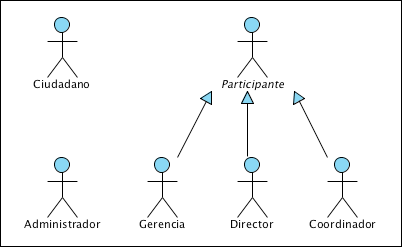
\includegraphics[width=.5\textwidth]{images/actores}
		\caption{Definición de actores del sistema.}
		\label{fig:actores}
	\end{center}
\end{figure}

%---------------------------------------------------------
\section{Alcance del prototipo}

%---------------------------------------------------------
\subsection{Cambios a la versión inicial}

	Los cambios a realizar sobre la Configuración inicial se resumen a continuación.

\begin{cambios}
	\PFCitem{PFC1 }{CU A1 Gestión de Usuarios}{\actualizar}
	\PFCitem{PFC2 }{CU A2 Gestión de Contactos}{\actualizar}
	\PFCitem{PFC2 }{CU A2.4 Gestión de Tipos de Contactos}{\actualizar}
	\PFCitem{PFC3 }{CU A3 Gestión de Tipo de Unidad}{\eliminar}
	\PFCitem{PFC4 }{CU A4 Gestión de Unidad}{\actualizar}
	\PFCitem{PFC5 }{CU A5 Gestión de Indicador}{\programar}
	\PFCitem{PFC6 }{CU A6 Gestión de Tipo de aviso}{\programar}
	\PFCitem{PFC7 }{CU A7 Gestión de Area}{\actualizar}
	\PFCitem{PFC8 }{CU A8 Gestión de Avisos}{\programar}
	\PFCitem{PFC9 }{CU A9 Gestión de Perfiles}{\eliminar}
	\PFCitem{PFC10}{CU A10 Gestión de Grupo}{\reemplazar{CU D Definir Estructura}}
	\PFCitem{PFC11}{CU A11 Gestión de Capitulo}{\reemplazar{CU A}}
\end{cambios}

Todos los cambios deben realizarse con base en las definiciones y consideraciones de este documento.

\subsection{Requerimientos que se agregan}

\subsection{Administración}
\begin{requerimientos}
	\FRitem{CU A12}{Gestión de proyectos Preregistrados}{Se consultan los proyectos preregistrados para su aprobación (con el registro del director responsable correspondiente) o su eliminación del sistema.}{}
\end{requerimientos}

\subsection{Gerencia}
\begin{requerimientos}
	\FRitem{CU G1}{Gestión de Programas}{Registro y actualización de los niveles y la estructura jerárquica del Programa de primer nivel.}{}
\end{requerimientos}

\subsection{Dirección}
\begin{requerimientos}
	\FRitem{CU D1}{Gestionar Programas de primer nivel}{Registro y actualización de información referente a los Programas de primer nivel y asignación de los directores correspondientes.}{}
	\FRitem{CU D2}{Gestión de Temas transversales}{Registro y actualización de los Temas transversales que aplican a todos los Programas de primer nivel.}{}
	\FRitem{CU D3}{Gestión de Ejes temáticos}{Registro y actualización de los Ejes temáticos que aplican a todos los Programas de primer nivel.}{}
\end{requerimientos}

\subsection{Coordinación}
\begin{requerimientos}
	\FRitem{CU C1}{Gestión de proyectos}{Consulta de proyectos registrados y preregistrados y preregistro de nuevos proyectos (esta ultima parte es con o sin cuenta de usuario).}{}
\end{requerimientos}

\subsection{Otro}
\begin{requerimientos}
	\FRitem{CU 0}{Control de acceso}{Inicio y cierre de sesión de todos los usuarios del sistema.}{}
\end{requerimientos}

%=========================================================
\chapter{Proceso de negocios}


%---------------------------------------------------------
\section{Proceso}

\begin{figure}[htbp!]
	\begin{center}
		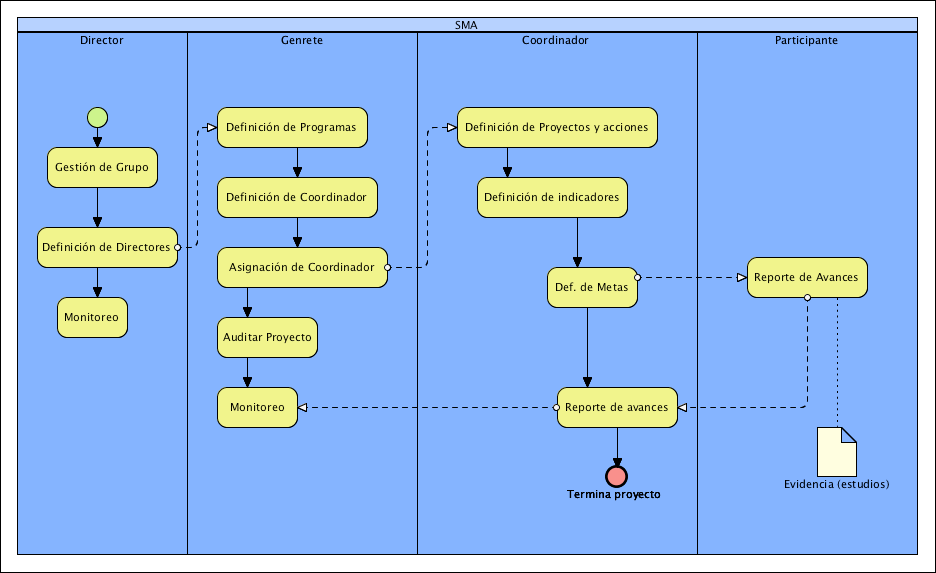
\includegraphics[width=.8\textwidth]{images/proceso}
		\caption{Proceso para el registro y definición de proyectos.}
		\label{fig:default}
	\end{center}
\end{figure}

%---------------------------------------------------------
\section{Reglas de Negocio}

\Instrucciones{Reglas de negocio: definición, hecho, afirmacion sobre un echo, restriccion, cálculo.}
\cfinput{reglas}


%=========================================================
\chapter{Modelo del comportamiento}

%---------------------------------------------------------
\section{Diagrama de CU}

\begin{figure}[htbp!]
	\begin{center}
		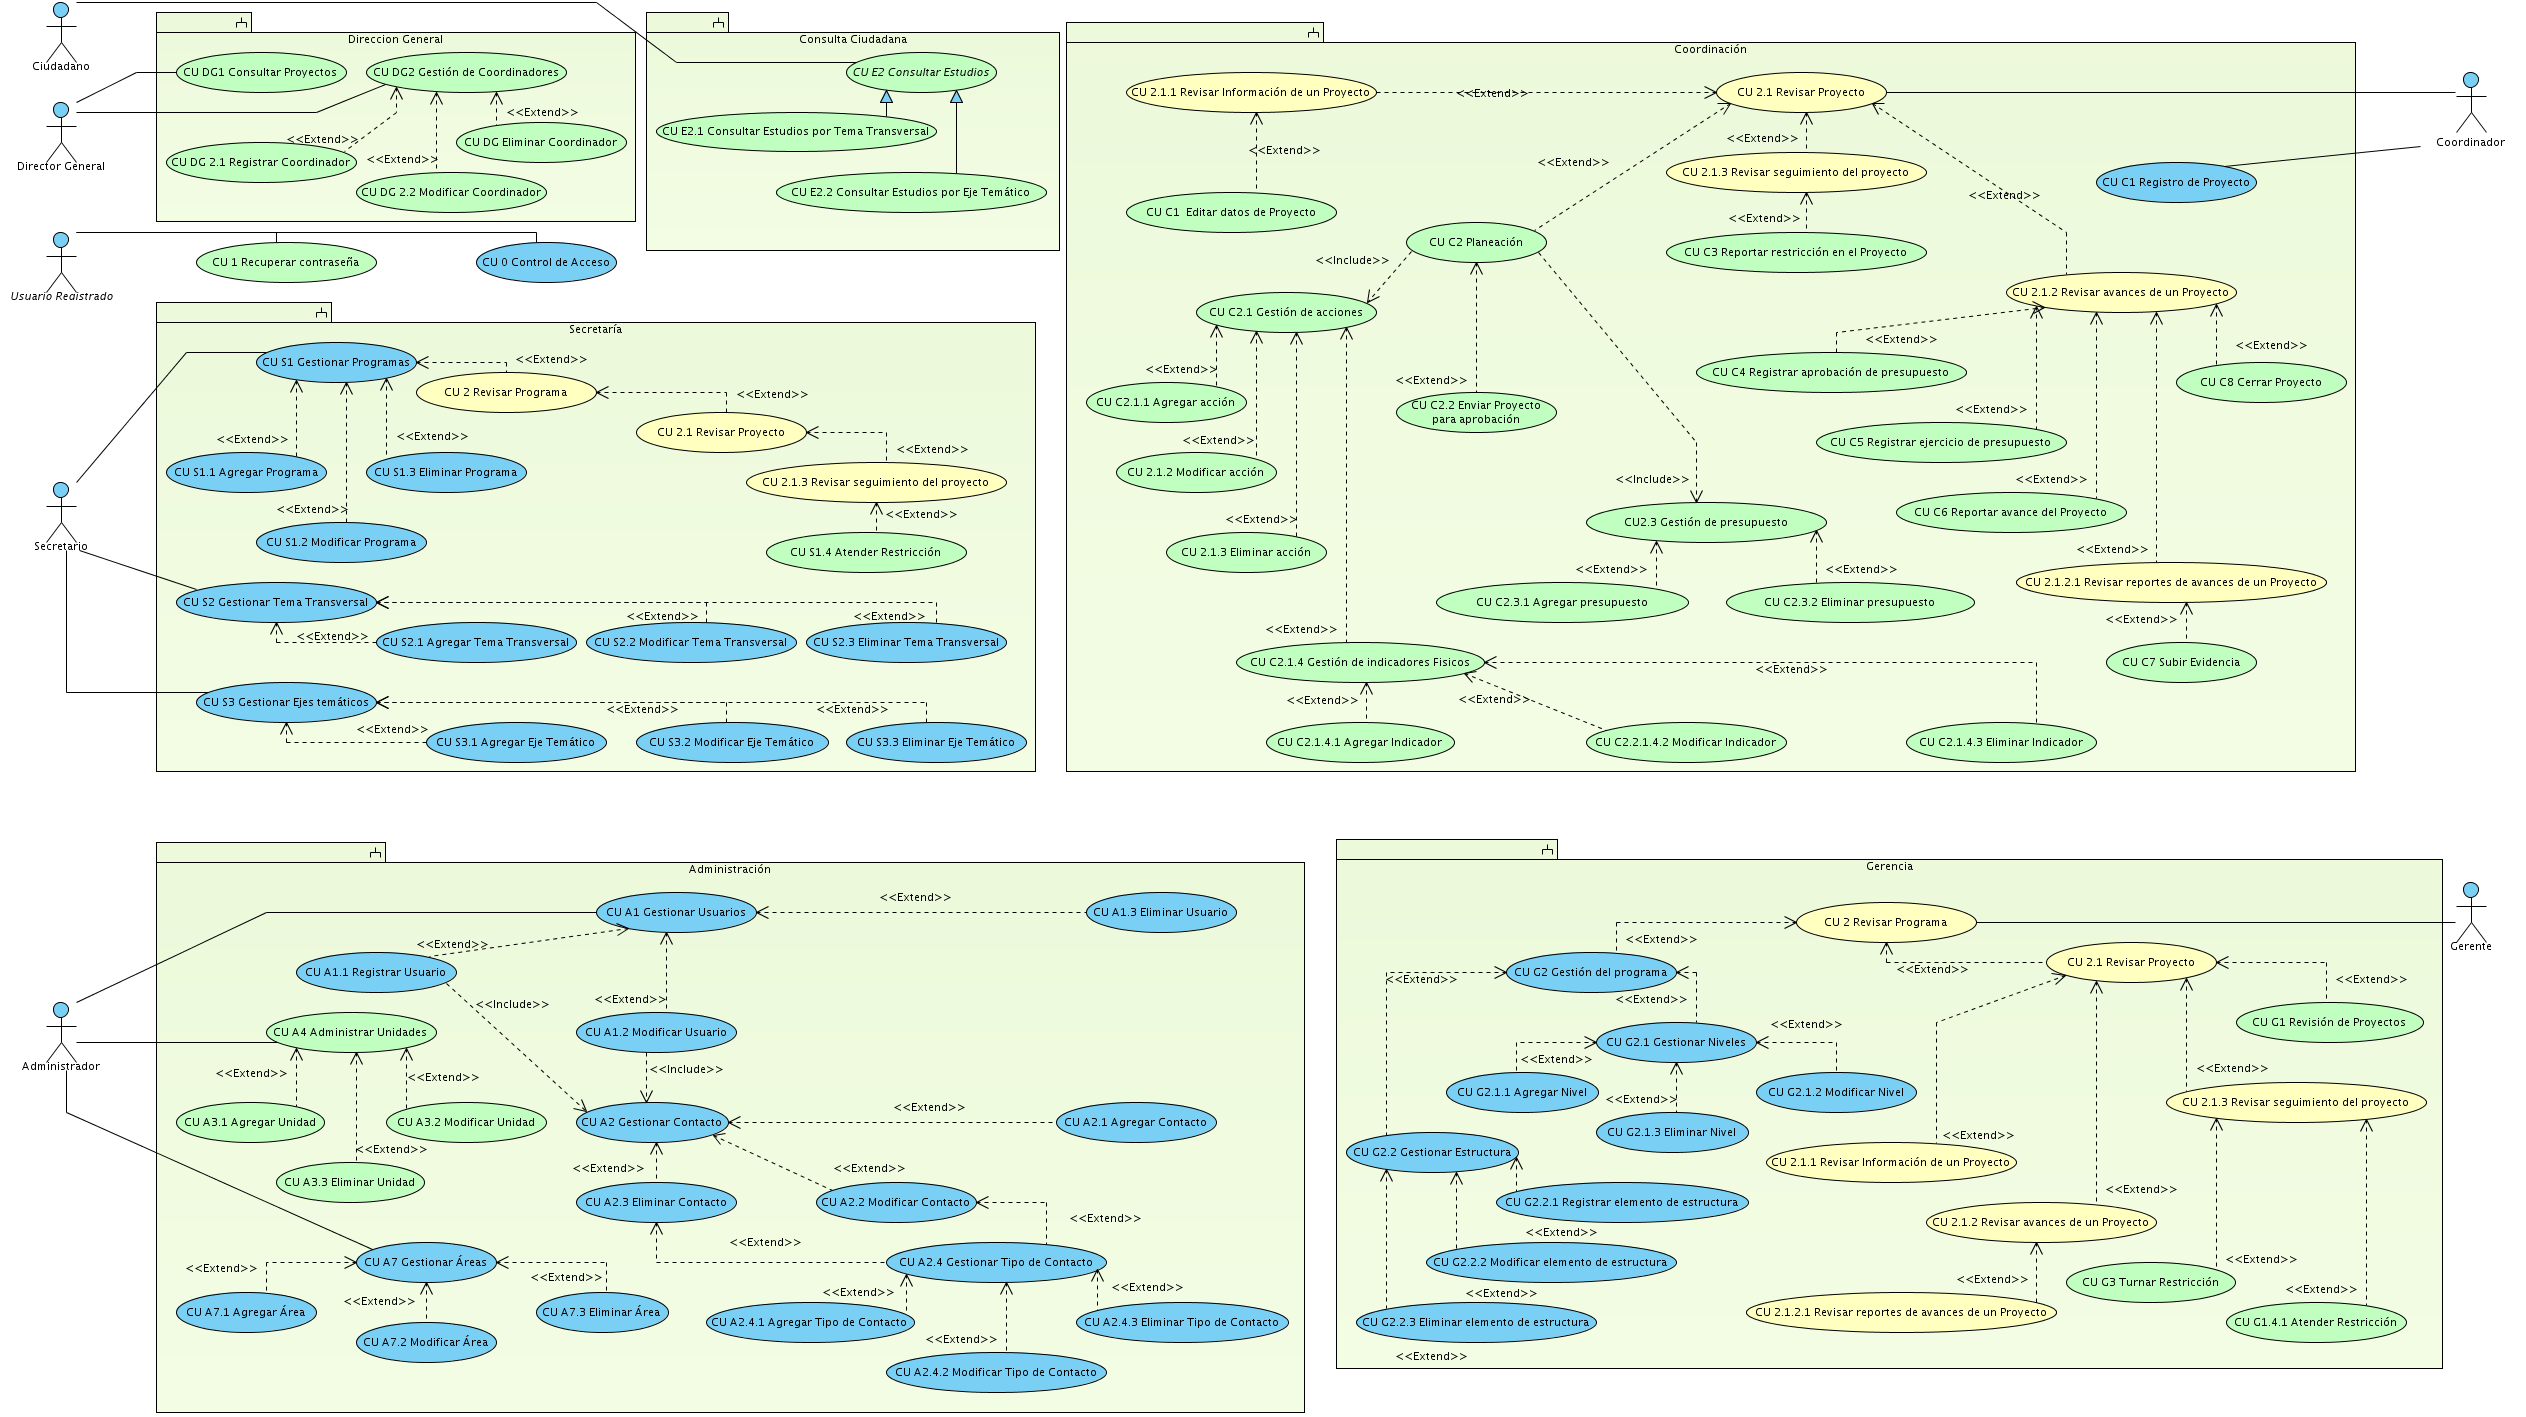
\includegraphics[angle=90,height=\textheight]{images/casosDeUso}
		\caption{Casos de uso del prototipo}
		\label{fig:default}
	\end{center}
\end{figure}

%=========================================================
\chapter{Modelo detallado del comportamiento, Control de acceso} 

%----------------------------------------------------------
\section{Diagrama de casos de uso}

\begin{figure}[htbp!]
	\begin{center}
		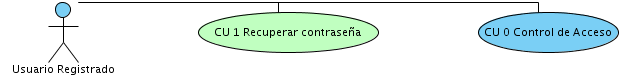
\includegraphics[width=.3\textwidth]{images/CUcontrolAcceso}
		\caption{Casos de uso para el control de acceso}
		\label{fig:default}
	\end{center}
\end{figure}

\cfinput{cu0iniciar_sesion/cu}


%%======================================================================\chapter{Modelo del dominio del problema} 

\section{Diagrama Entidad/Relación}

  	\begin{figure}[h!]
 		\centering
 			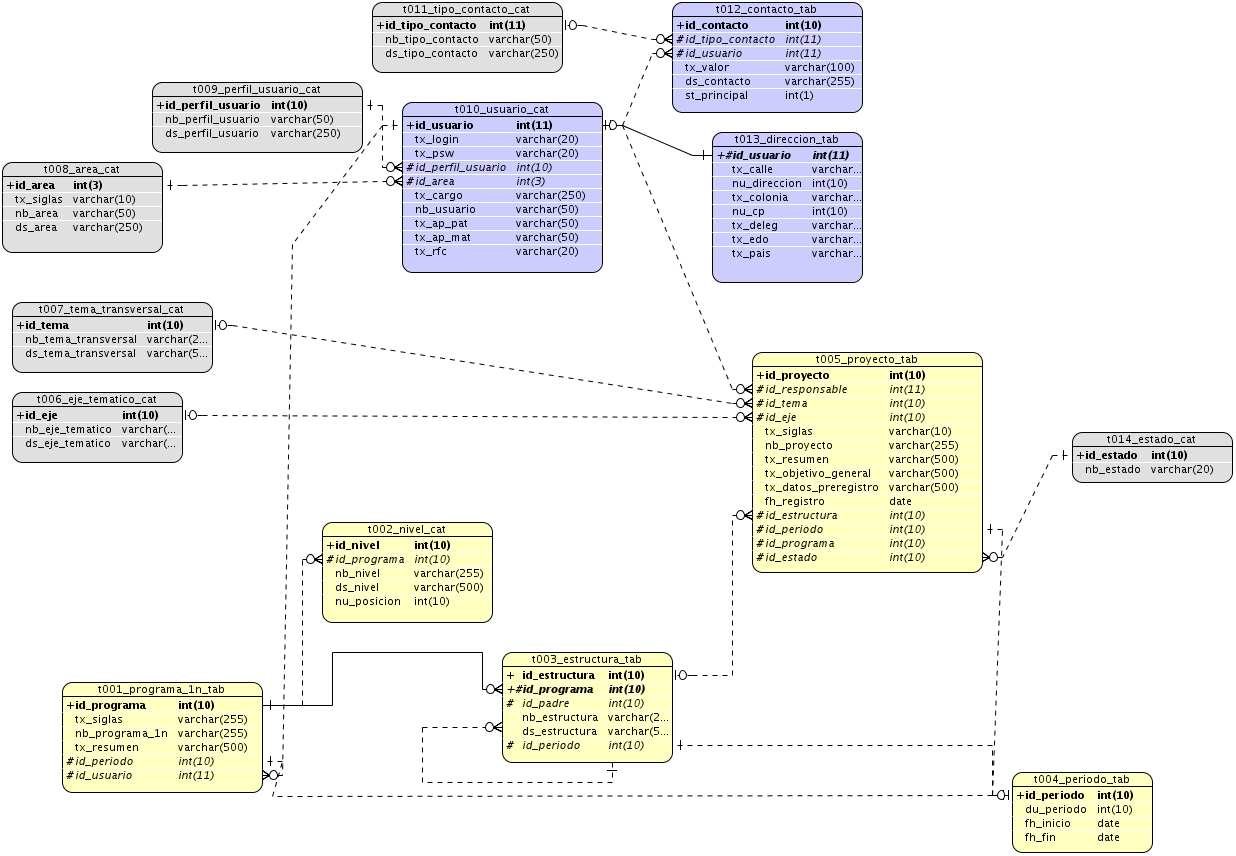
\includegraphics[width=.8\textwidth]{images/modeloER}
 		\caption{Unidad}
 	\end{figure}

\section{Diccionario de Datos}

\cfinput{diccionario}



\end{document}
